\documentclass[onecolumn]{aastex62}

%%
\usepackage{minted}
\usepackage{wrapfig}
\usepackage{appendix}
\newcommand{\vdag}{(v)^\dagger}
\newcommand\aastex{AAS\TeX}
\newcommand\latex{La\TeX}
\newcommand{\ha}{H$\alpha$ }
\graphicspath{{./}{figures/}}
\defcitealias{MBK2017}{B17}


\shorttitle{SAM Globular Clusters}
\shortauthors{Pearce, L.}

\begin{document}

\title{``Well, it was an idea": Millennium simulation is insufficient to reproduce known globular cluster/dark matter halo mass relations}


\author{Logan Pearce}
%\affiliation{Department of Astronomy, University of Texas at Austin, Austin, TX, 78712, USA}

%\begin{abstract}

%\end{abstract}


\section{Introduction} \label{sec:intro}
Globular clusters (GCs) are unarguably the prettiest things to look at at a star party, and an important piece of the star-formation puzzle.  They are nearly universally old stellar populations, originally thought to be the result of a single starburst event, now shown to include several generations of star formation \citep[e.g.][]{Gratton2012}.  Their masses do not appear to correlate with the baryonic matter of the host galaxy, yet strongly correlate with the present-day dark matter (DM) halo mass \citep{Spitler&Forbes2009,Forbes2016,Harris2017,Forbes2018}, despite the fact there is no dynamical evidence for dark matter in GCs themselves \citep{Conroy2011}.  This linear correlation is so tight, it has been used as a method of measuring dark matter halo mass by observing the mass of GCs within the halo \citep[e.g.][]{Spitler&Forbes2009,Forbes2016}, because the ratio of $M_{\rm{GC}}$ to $M_{\rm{Halo}}$ is constant \citep{Spitler&Forbes2009,Harris2017}.  Metal-poor globular clusters are thought to form at high redshift \citep{Brodie2006}, so the connection between DM halo mass and GC system mass must be at high redshifts rather than present day.  Models of dark matter halo formation as a function of redshift thus can be used to test models of GC formation at high redshift (z $\gtrsim$ 5) which propagate to observable relations at present day (z=0).



\section{Method} \label{sec:method}
\subsection{Model for GC formation}
In this study, I modified the class semi-analytic model to form and evolve globular clusters, and tune model parameters to reproduce observational results.  To introduce globular cluster formation to the semi-analytic model, I relied on the simple model for forming GCs supplied by \cite{MBK2017} (hereafter \citetalias{MBK2017}).  \citetalias{MBK2017} develops a purely phenomenological simple analytic model for the formation of GCs that depends solely on the dark matter halo mass, and applies his model to merger trees from the \cite{Planck2016} to reproduce results and discuss implications.  His model is effective solely based on its ability to reproduce observational results, not on detailed physics of GC formation.

To summarize briefly, the model works on a the simple assumption that the mass in GCs scales linearly with the mass of the dark matter halo at a single epoch of formation, which is z$\sim$6.  At z=6, any DM halo above a certain minimum halo mass for forming GCs (M$_{\rm{min}}$) will form them according the formula
\begin{equation}
    \langle M_{\rm{GCs}} | M_{\rm{Halo}}(z=6) \rangle = \langle m_{\rm{GC}}(z=6)\rangle \frac{M_{\rm{halo}}}{M_{\rm{min}}} f\big( \frac{M_{\rm{halo}}}{M_{\rm{min}}} \big)
\end{equation}
where $\langle M_{\rm{GCs}} | M_{\rm{Halo}}(z=6) \rangle$ is the average total mass in GCs in a halo at z=6, $\frac{M_{\rm{halo}}}{M_{\rm{min}}}$ is the ratio of that halo's mass to the minimum mass for forming GCs, $f\big( \frac{M_{\rm{halo}}}{M_{\rm{min}}} \big)$ is a suppression function of the halo/min mass ratio, and $\langle m_{\rm{GC}}(z=6)\rangle$ is the average mass of a single globular cluster at z=6.  Following the epoch of GC formation, the total mass in a halo that is in GCs is simply a function of the progenitor halos that were above the $M_{\rm{min}}$ at z=6.  So the total mass in a halo at z=0 is the sum of all the GCs in progenitor halos:
\begin{equation}
    \langle M_{\rm{GCs}} | M_{\rm{Halo}}(z=0) \rangle = \sum_i \langle M_{\rm{GCs}} | M^i_{\rm{Halo}}(z=6) \rangle
\end{equation}
where i is a progenitor halo of the halo at z=0.

Several assumptions are involved in this model.  Here I have summarized the essential model assumptions I adopted for my analysis, and do not entirely replicate the list found in \citetalias{MBK2017}; see that reference for the complete list off assumptions used in developing the model. 
\begin{enumerate}
    \item Following \cite{Harris2017}, the average GC mass at present time  is assumed to be constant at $\langle m_{\rm{GC}}(z=0)\rangle = 2.5 \times 10^5 \;\rm{M}_\odot$, and the present day GC mass is smaller than its mass at formation by some factor $\xi$, where
    \begin{equation}
        \xi  \equiv \frac{\langle m_{\rm{GC}}(birth)\rangle}{\langle m_{\rm{GC}}(z=0)\rangle}
    \end{equation}

    \item The total mass in present day GCs is a constant fraction of the dark matter halo mass:
    \begin{equation}
        \langle M_{\rm{GCs}} | M_{\rm{Halo}}(z=0) \rangle = \eta  M_{\rm{Halo}}(z=0)
    \end{equation}
    with $\eta = (3-4) \times 10^{-5}$ \citep[e.g.][]{Harris2017}
    
    \item \citetalias{MBK2017} derives $M_{\rm{min}}\approx 1.07\times10^{9} \rm{M}_\odot$

\end{enumerate}

\subsection{Implementation of the simplest form of the GC formation model}
To implement this model into the class semi-analytic model (SAM), I made two simple additions to the existing code (for to complete script with code annotations, see Appendix).  First, I added an \texttt{if} statement to apply the GC formation treatment only if a halo in the tree is at the epoch of GC formation, z=6.  At that epoch, if the halo is at or above the minimum mass, then form GCs in that halo according to Eqn (1).  In the simplest case, I used the following form of the function f:
\begin{equation}
    f = \left\{ \begin{array}{rcl}
        1 & \mbox{for}
        & \frac{M_{\rm{halo}}}{M_{\rm{min}}} \ge 1 \\ 
        0 & \mbox{for} & \frac{M_{\rm{halo}}}{M_{\rm{min}}} < 1\\
        \end{array}\right.
\end{equation}
which effectively turns on GC formation if the minimum mass is exceeded, and turns it off if the halo mass is below the minimum mass.  Below is the code snippet added to the class semi-analytic model within the for loop (bginning at line 343 of code in Appendix):
\begin{minted}[mathescape, linenos]{python}

    # If the halo is at the epoch of GC formation, form GCs according to MBK2017 model:
    if scale == z6_scale:
        # If the halo mass is greater than M_min:
        # (convert from Msun/h to Msun before comparing)
        if trees[x]['mvir']/h > M_min:
            # compute the average total mass in globular clusters:
            # <M_GC|M_halo(z=6)> = <m_GC(z=6)> * (M_halo/M_min)
            avg_mass_in_GC_z6 = avg_z6_GC_mass * ((trees[x]['mvir']/h) / M_min)
            # add to tree:
            trees[x]['m_GC'] = avg_mass_in_GC_z6
            trees[x]['N_GC'] = ((trees[x]['mvir']/h) / M_min)
\end{minted}

Second, to propagate the GC mass forward in time to z=0, I created a separate function after the SAM run is complete.  This function runs through each halo at z=0, and finds all z=6 halos that ended up in that halo at z=0, and sums the mass (Eqn (2)).  
\begin{minted}[mathescape, linenos]{python}
def get_z0_GC_mass(trees):   
    z0_halos = [trees[x] for x in halos_at_scale[1]]
    z6_halos = [trees[x] for x in halos_at_scale[z6_scale]]
    # For each z=0 halo:
    for j in range(len(z0_halos)):
    # look through all the z=6 halos:
        for i in range(len(z6_halos)):
        # If the Tree Root ID matches the z=0 root id:
            if z6_halos[i]['Tree_root_ID'] == z0_halos[j]['Tree_root_ID']:
            # sum the mass into the z=0 GC mass:
                z0_halos[j]['m_GC'] += z6_halos[i]['m_GC']
        update_progress(j,len(z0_halos))
\end{minted}

\subsection{Assessing Model Performance}
To test the performance of the model, I selected a few results which serve as observational tests of GC formation.

\citealt{Spitler&Forbes2009} use observations of GC mass and luminosity to derive the mass of the halo, essentially working backwards compared to what I am doing with this model.  They derive observationally that the halo mass is 4.15 dex larger than the total GC mass, that is:  
\begin{equation}
    log\big(\frac{M_{halo}}{M_\odot}\big) = log\big(\frac{M_{GCs}}{M_\odot}\big) + 4.15
\end{equation}
which makes a good test of the model if it can recover this relation.  

A second observational test is the value of $\eta$ from Eqn (4).  \cite{Harris2017} find $\eta = 2.9 \times 10^-5$, while \cite{Forbes2016} find $\eta = 3.4 \times 10^-5$, both from observational studies.  \cite{MBK2017} assumes a constant value of $\eta(M_{halo})$ in developing his model, so the ability for my SAM to recover the correct $\eta$ serves as a test of the model.

\subsection{Tune-able parameters}\label{sec:params}
Even though the model is simple, there are a few avenues for tuning it to match observations.  \citetalias{MBK2017} suggests a suppression function that is 1 for $M_{\rm{halo}}(z=6) > M_{\rm{min}}$ and exponentially decreasing for $M_{\rm{halo}}(z=6) < M_{\rm{min}}$.  The value of $M_{\rm{min}}$ can be fine-tuned as well to adjust which halos form GC at z=6.  Additionally, \citetalias{MBK2017} provides a relation between $M_{\rm{min}}$ and redshift, which could be employed.  Finally, the value of $\xi$ (Eqn 3) is a free-parameter in \citetalias{MBK2017}, and can be adjusted to fine-tune the scale factor of the \citealt{Spitler&Forbes2009} relation.

\begin{figure*}[!htb]
\centering
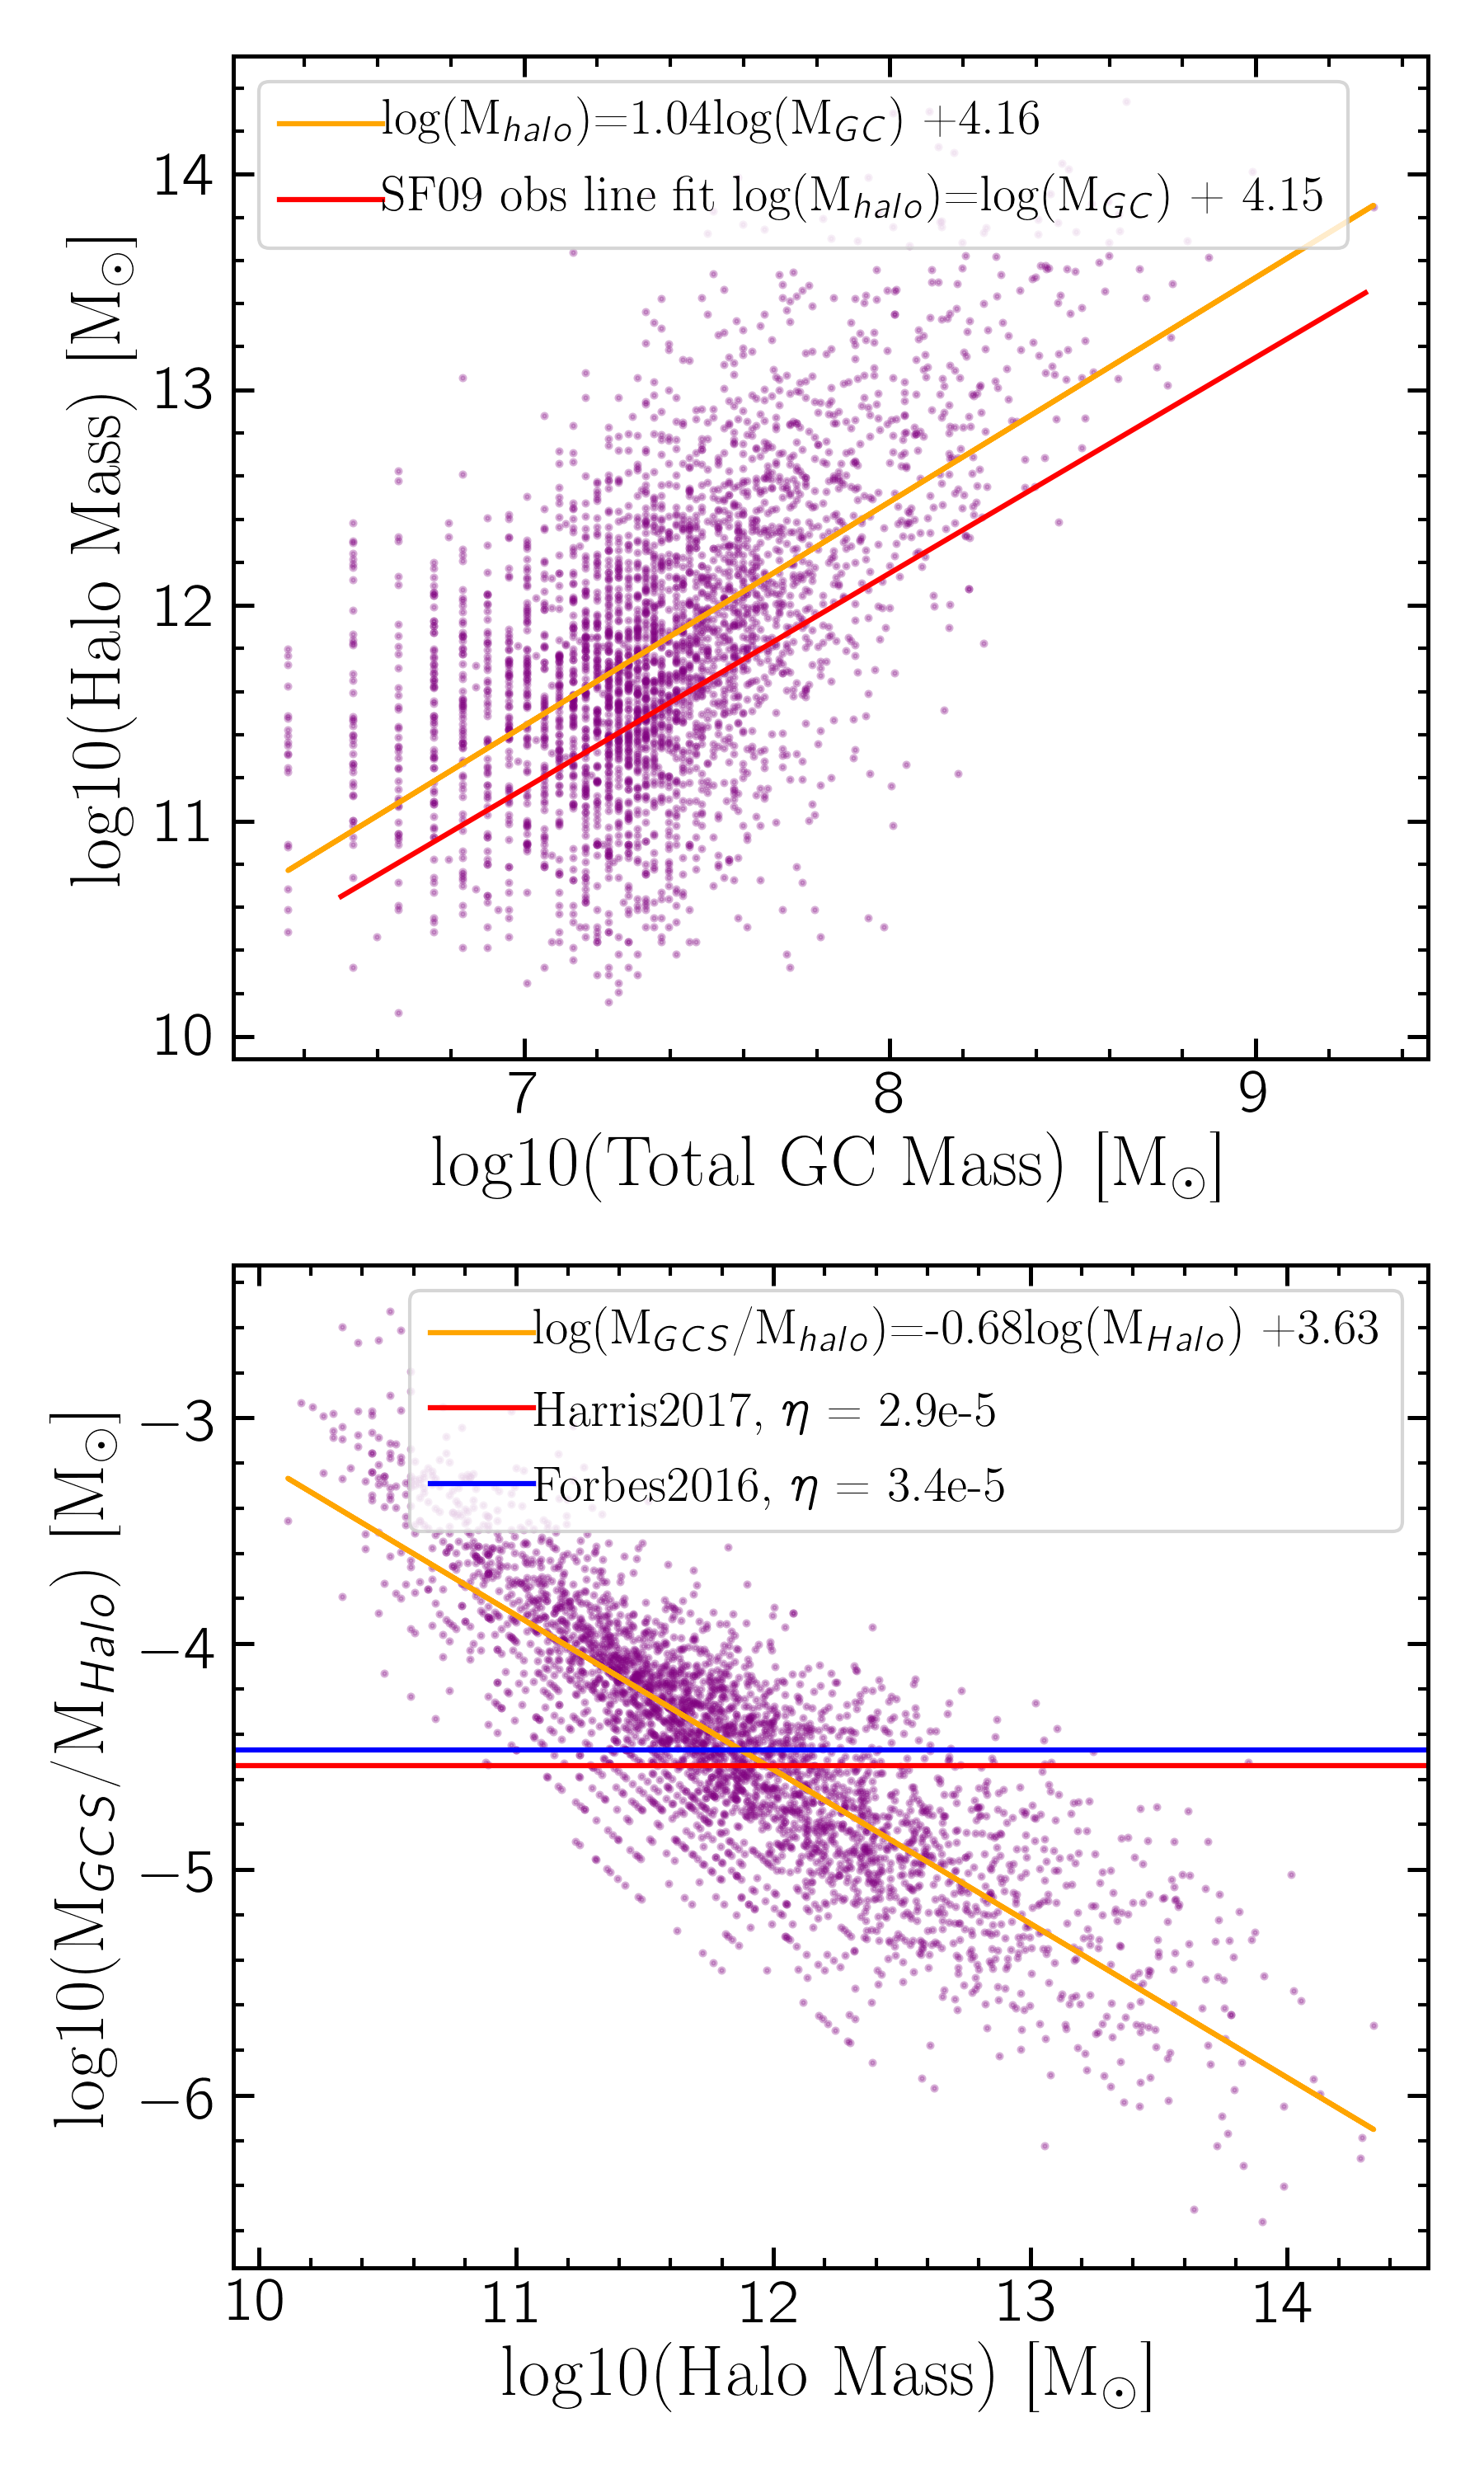
\includegraphics[width=0.3\textwidth]{GCtest_initial_simple.png}
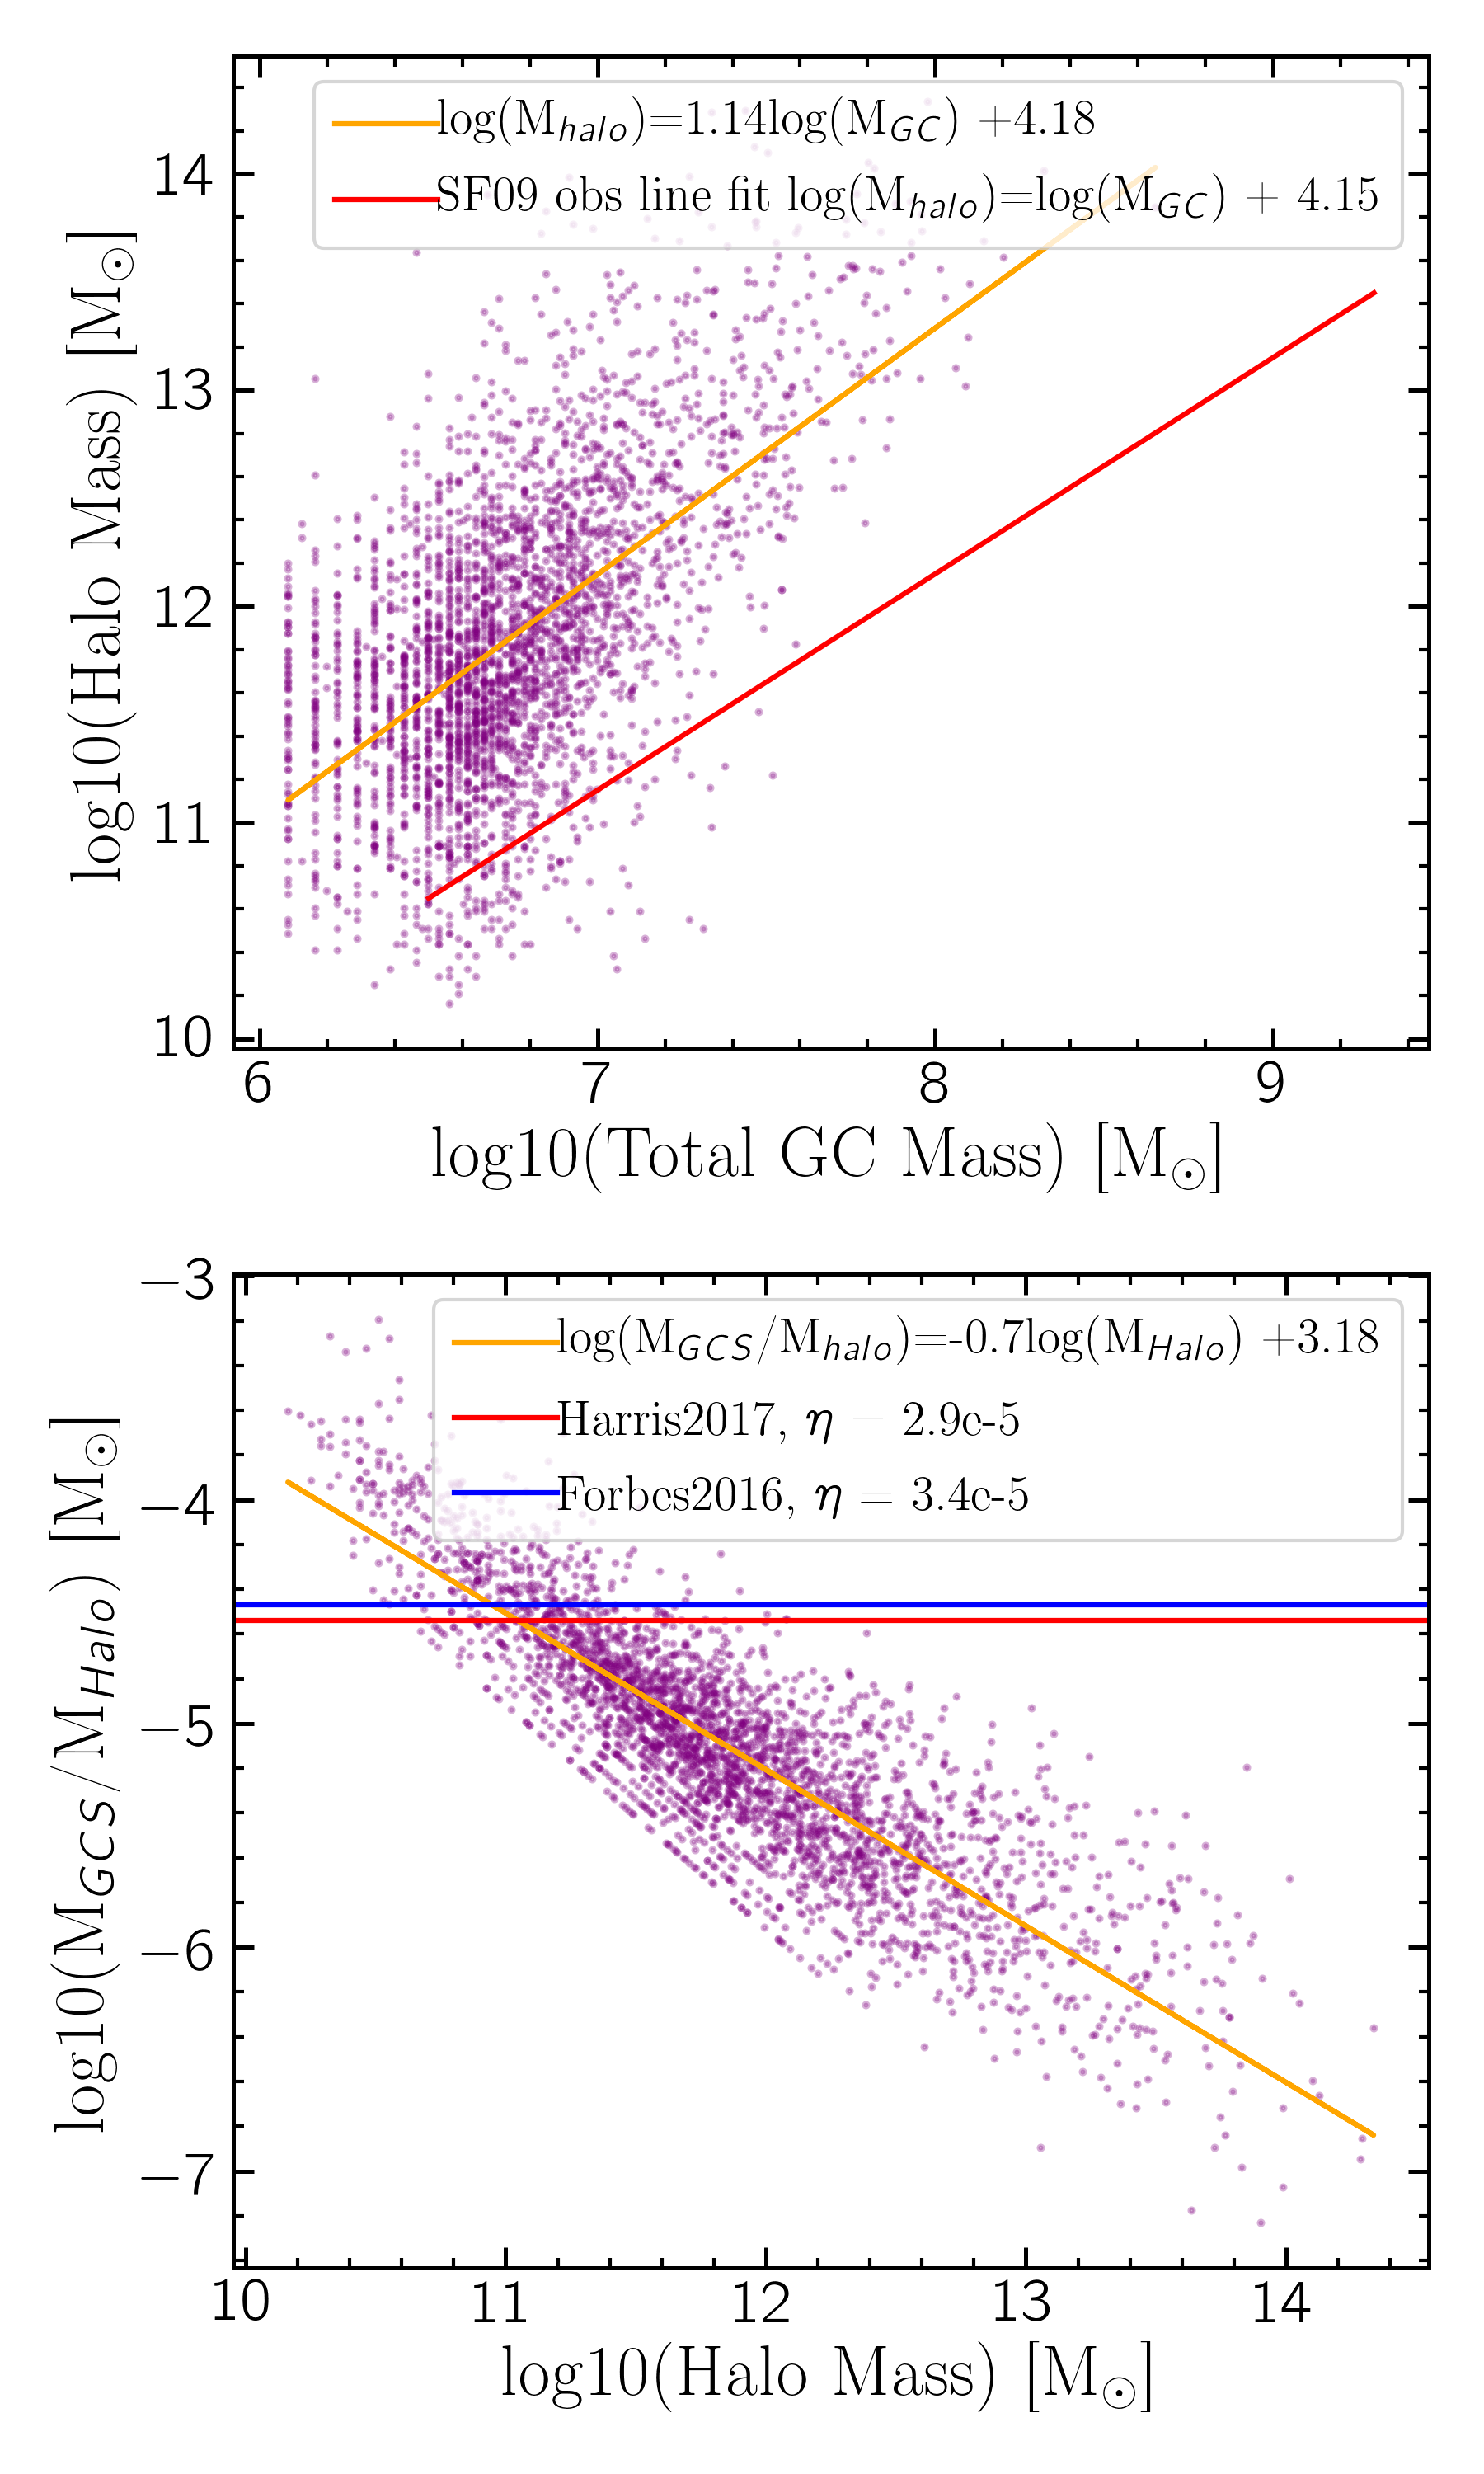
\includegraphics[width=0.3\textwidth]{GCtest_tree_Mmin_5e9.png}
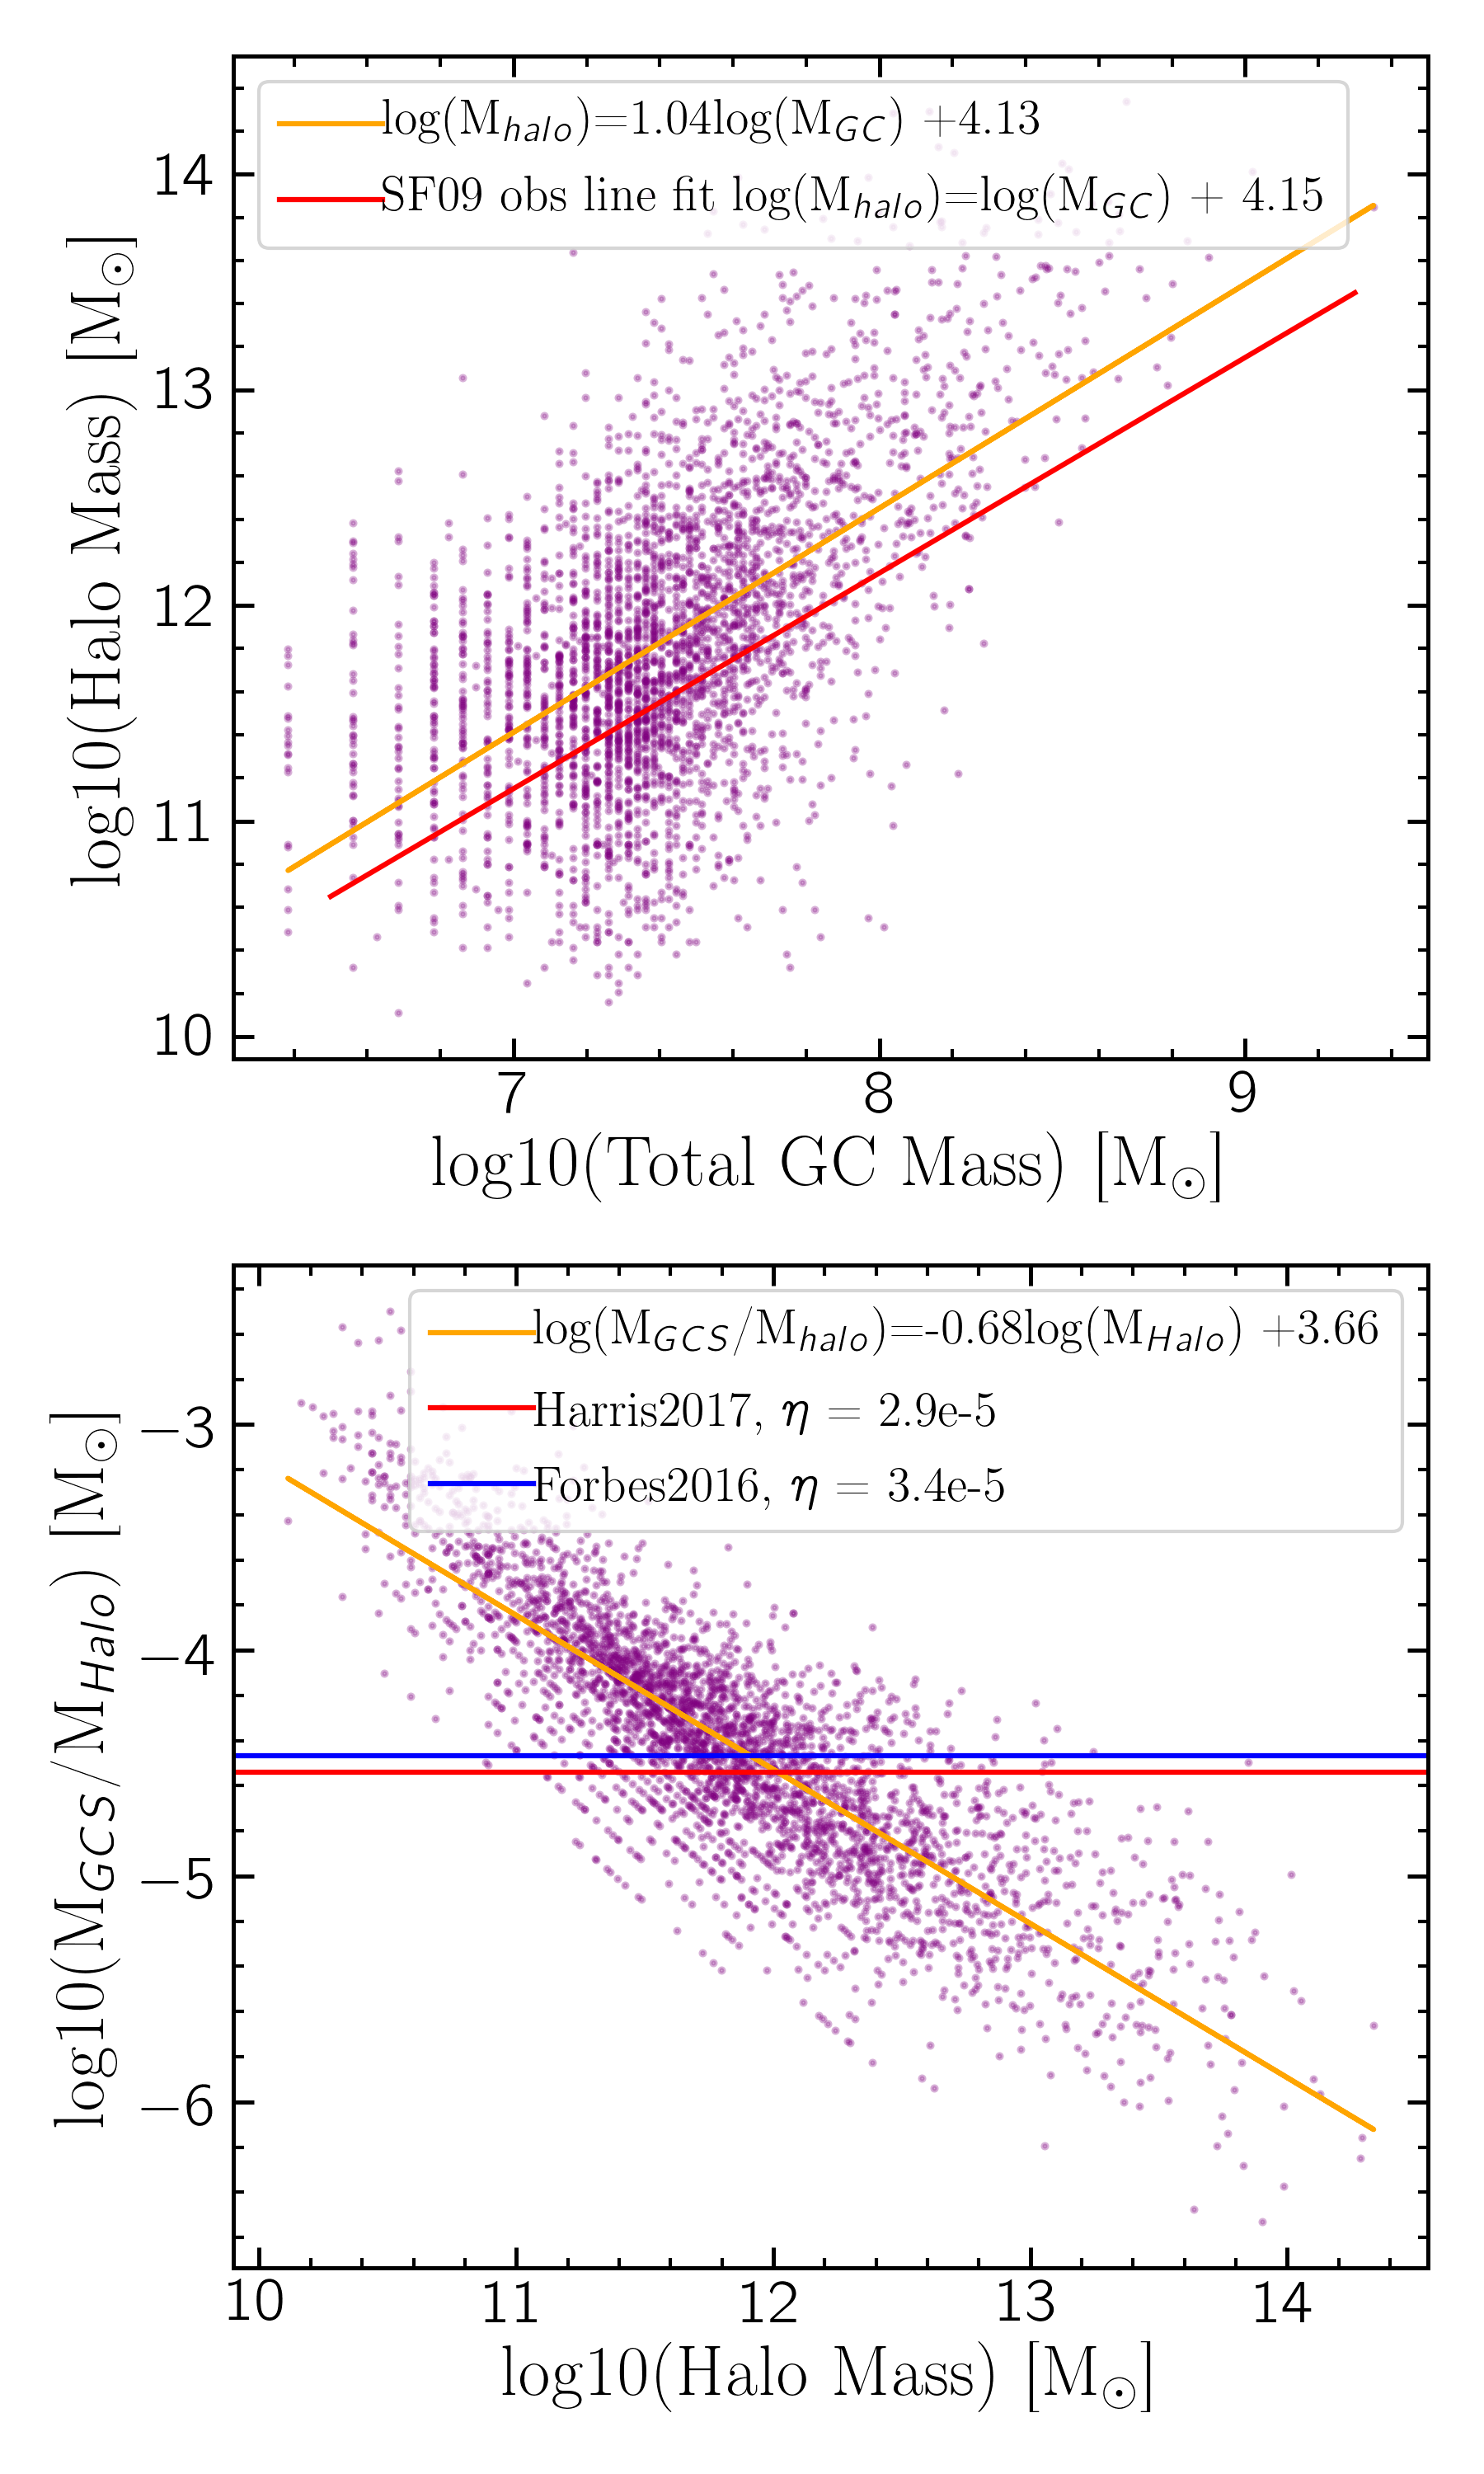
\includegraphics[width=0.3\textwidth]{GCtest_tree_varying_minmass.png}
\caption{\small{Top: Tests of varying parameters against \cite{Spitler&Forbes2009}.  Purple scatter points are individual z=0 halos with GCs; the orange line is a linear regression fit to the purple points; the red line is the relation of \cite{Spitler&Forbes2009}.  Bottom: tests of the value of $\eta$.  purple and orange are smae as above; horizontal lines indicate values of $\eta$ from \cite{Harris2017} (red) and \cite{Forbes2016} (blue).
Left: Initial test of most simple model, with $M_{\rm{min}} = 1.07e9 M_\odot$, $\xi = 3$.  The relation of \cite{Spitler&Forbes2009} is nearly reproduced, however $\eta$ has a decreasing relation with halo mass.  Center: test with $M_{\rm{min}} = 5e9 M_\odot$.  The resulting fit is further from \cite{Spitler&Forbes2009}, as is the $\eta$ relation.  Right: Test with $M_{\rm{min}}(z)$ according to \citetalias{MBK2017} Fig 3.  The result is effectively unchanged from the initial test.}}
\label{fig:initial_results}
\end{figure*}

\section{Results \\ -or- \\Things Did Not Go According to Plan.}
Results of some initial tests varying parameters discussed in Section \ref{sec:params} are shown in Figure \ref{fig:initial_results}. I performed an initial run with the simple suppression function (Eqn 5) and $\xi=3$ as an initial starting guess.  We see in Figure \ref{fig:initial_results}(left, top) that the relation of \cite{Spitler&Forbes2009} is nearly reproduced despite the scatter, which is significantly larger than theirs.  The slope of the line is 1.5$\sigma$ from their value, and the y-intercept is 0.07$\sigma$.  These were initially very promising results.  However as Figure~\ref{fig:initial_results}(left, bottom) shows, the value for $\eta$ is problematic.  While the median of the scatter distribution is spot-on at $\eta = 3.6 \times 10^-5$, there is a decreasing trend of $\eta$ with halo mass.  This indicates that while the model is rather successful at coming close to reproducing results, there are issues at high and low halo mass regimes.

I proceeded with testing the parameters in Section \ref{sec:params} with no improvement in results.  The value of $\xi$ serves as a scale factor for the mass of GCs formed.  While $\xi=3$ was initially very close, it did not really need to be refined further.  I found that  $\xi=3.1$ gave the y-intercept of 4.15, and did not change the value of the slope.  Figure \ref{fig:initial_results} center displays the results for adjusting $M_{\rm{min}}$, here set to $M_{\rm{min}} = 5\times10^9$.  Both fits were worse than the initial test.  Figure~\ref{fig:initial_results} right displays the result for implementing the minimum mass as a function of redshift according to \citetalias{MBK2017} Fig 3, which had essentially no impact on the results.  Establishing an exponential suppression function similarly had little effect on the results.  The reason is discussed further in Section~\ref{sec:discussion}.  


\section{Discussion \\ So what went wrong?}\label{sec:discussion}
The failure of my model to produce a constant $\eta(M_{\rm{Halo}})$ or to reproduce the small scatter of \citealt{Spitler&Forbes2009} Fig 3 ultimately is explained in the simulation resolution.  The SAM is built on the merger trees from the Millennium simulation, which has a mass resolution of $8.7\times10^9 \; M_\odot/h$.  This is larger than the minimum mass for forming GCs of $M_{\rm{min}} = 1.07 \times 10^9 M_\odot$.  Thus, at z=6 every halo exceeded the minimum mass and formed GCs.  This is why my tests on changing $M_{\rm{min}}$ had little to no effect on the result.

I examined only halos at z=6 that were massive enough to have many ($>$20) simulation particles at z=6, shown in Figure~\ref{fig:20 part}.  No effect on the problematic relations, we still do not obtain a constant value for $\eta$.  

\begin{figure}[!htb]
\centering
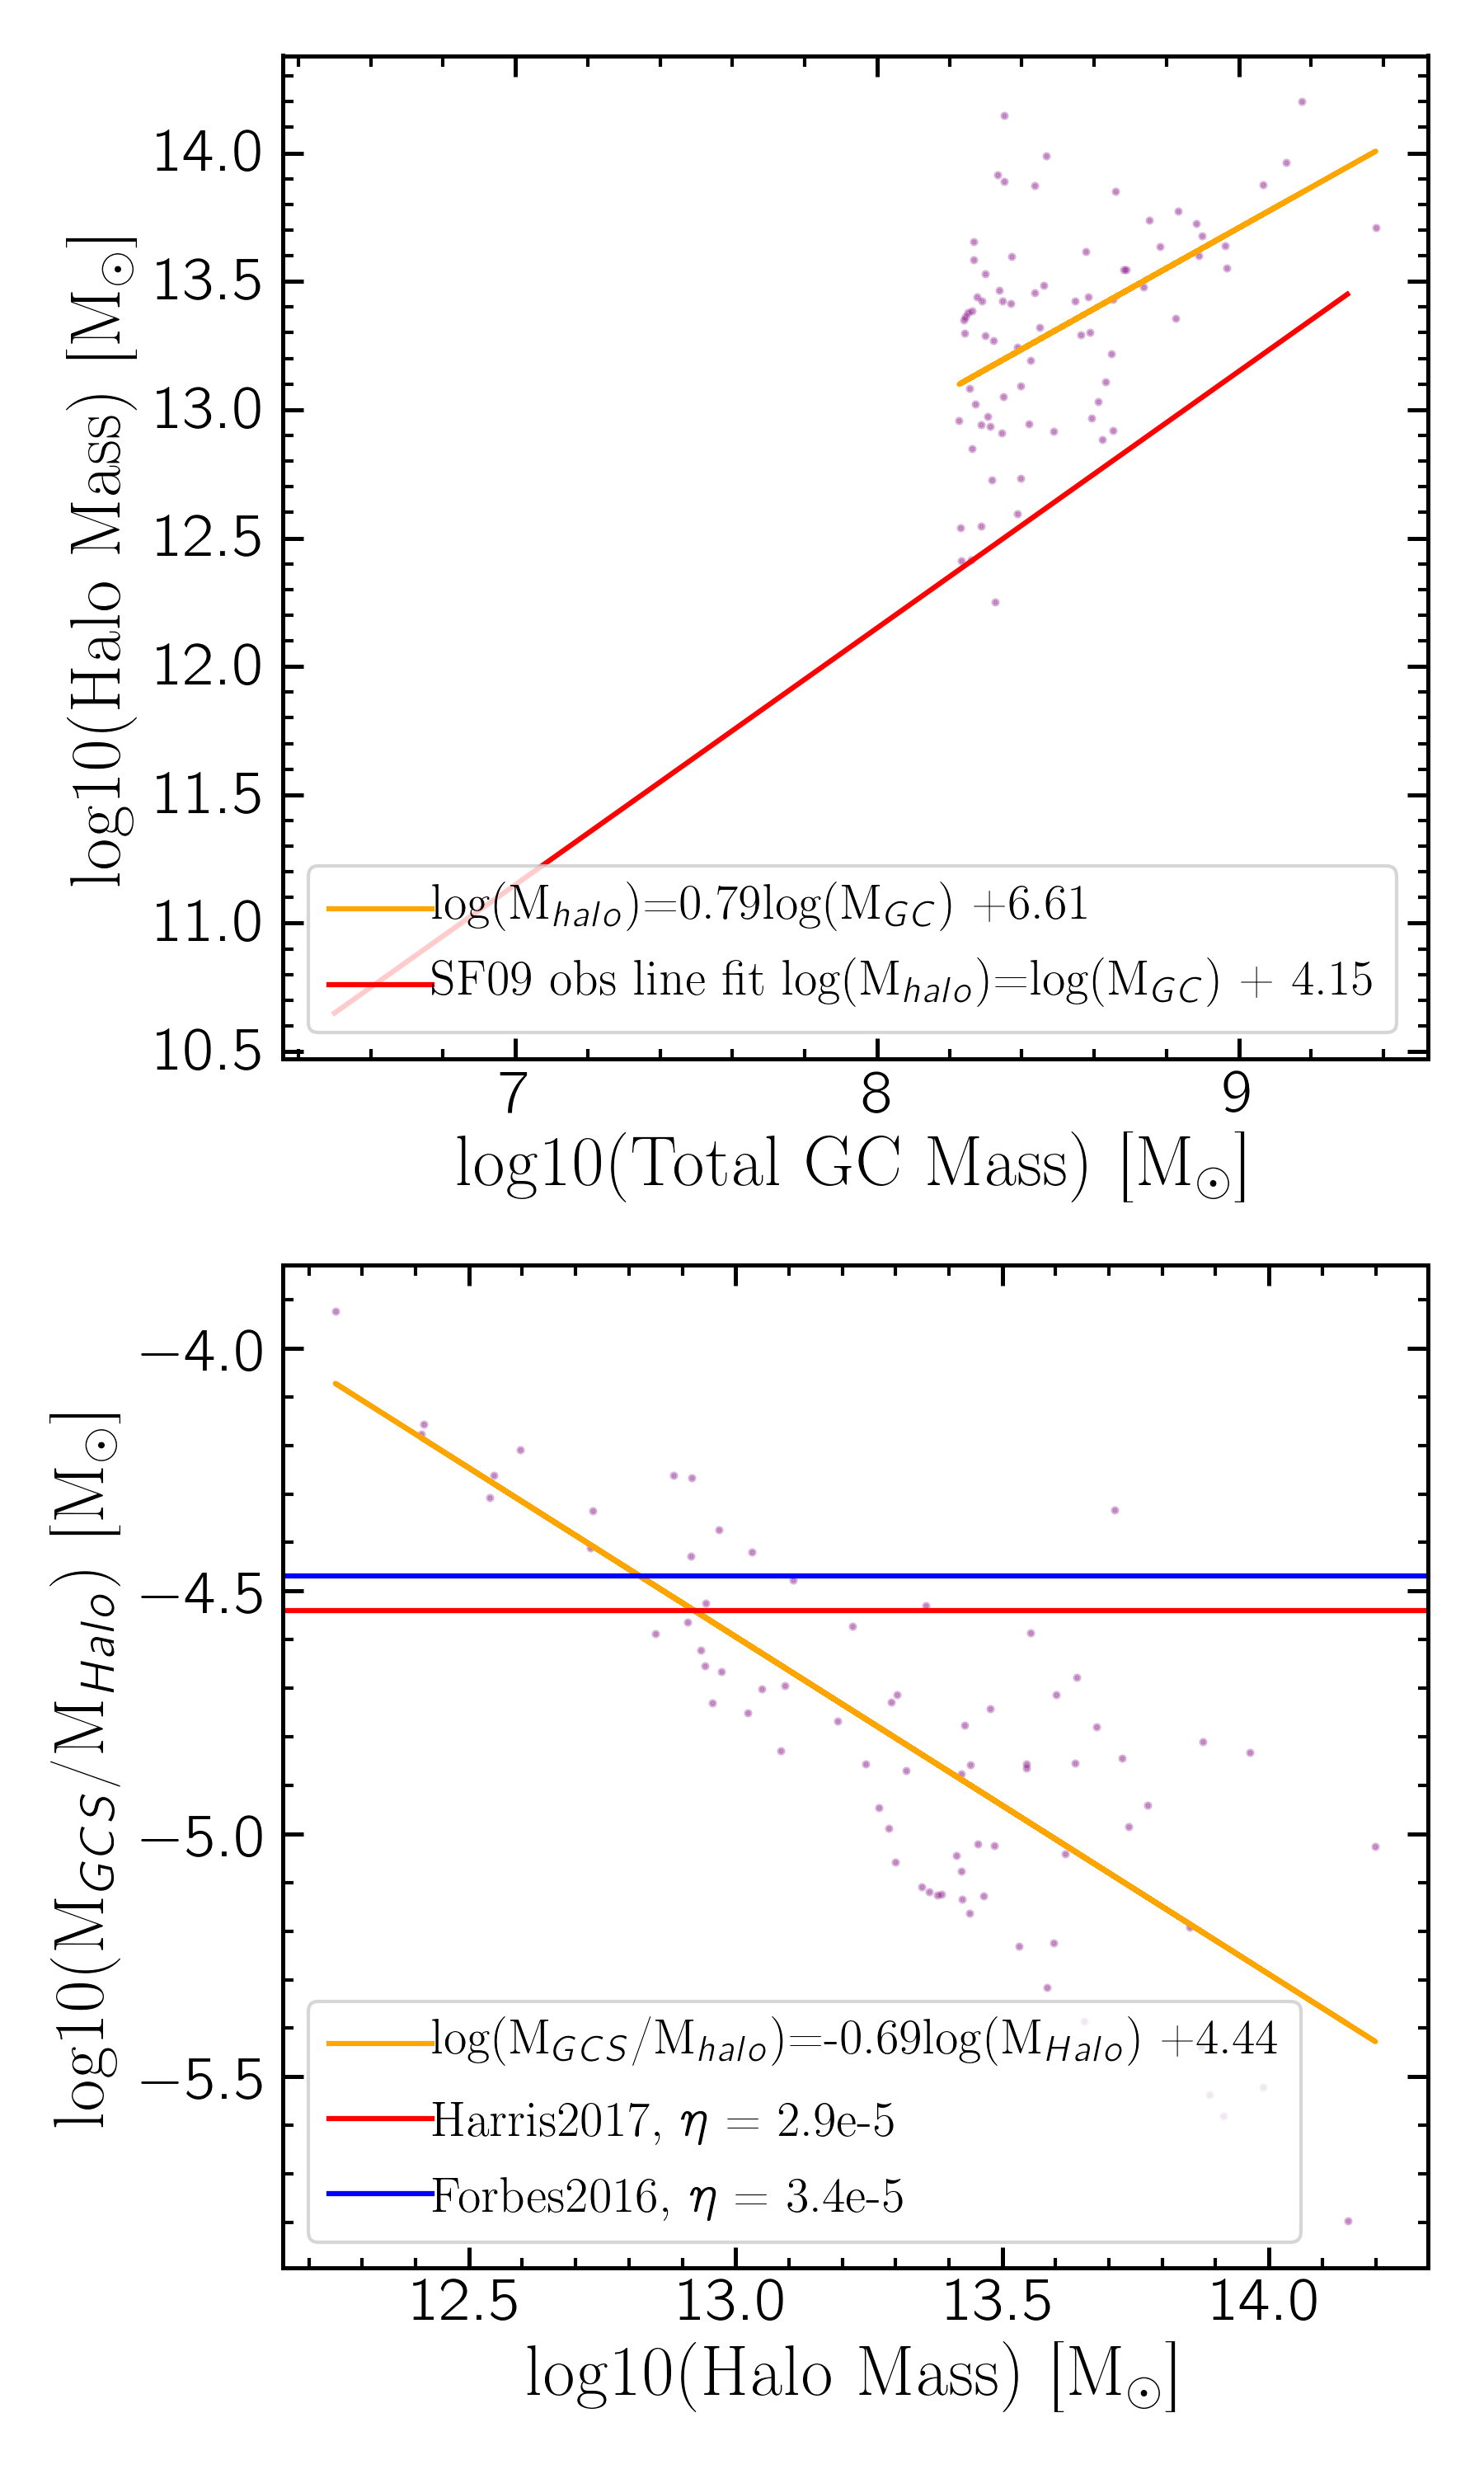
\includegraphics[width=0.3\textwidth]{GCtest_only_20_particles.png}
\caption{\small{Same plots as Figure 1, utilizing only z=6 halos with at least 20 simulation particles.  The same relationships as Figure 1 are retrieved.}}
\label{fig:20 part}
\end{figure}


Ultimately, in consultation with Dr. Boylan-Kolchin, I concluded this simulation is not capable of testing the \citetalias{MBK2017} GC formation model.  To have a meaningful test, and manipulation of parameters, a simulation with a higher mass resolution is required.  For example, the Millennium-II simulation \citep{Mill2} has a 125x higher mass resolution, with mass elements of $6.89\times10^6 M_\odot/h$, well below the minimum mass for GC formation.

Dr. Boylan-Kolchin noted an additional difficulty with using these merger trees.  My function used the \texttt{Tree\_root\_ID} to identify and retrieve all z=6 halos that went into a z=0 halo (see Section 2.2).  Dr. Boylan-Kolchin suggests that this retrieves only the central halo and not satellite halos, which might explain the dip in $\eta$ at higher halo masses.  Instead a "Friends of Friends" (FOF) ID parameter should be used, however the merger trees we are using do not include FOF IDs like the Millenium II simulation does.

\section{Conclusion}
I attempted to recreate the simple model for globular cluster formation of \citetalias{MBK2017} using the Millennium simulation merger trees and class-derived galaxy formation semi-analytic model, and use it to recreate the observed GC relationship with halo mass.  Ultimately, these merger trees were unable to reproduce observations due to the large mass resolution of the simulation.  In order to properly test the model, a higher resolution simulation should be used, such as the Millennium II simulation.



\bibliography{refs}


\appendix



\section{Semi-analytic model code}
This appendix shows the entire script used to make the semi-analytic model.  The SAM function begins on line 288, with detailed docstring describing the function and arguments.  All comments in the SAM function denote and describe changes to the model beyond what was done in class to accomplish the globular cluster formation, which begins on line 344; uncommented sections are the same as they were in class.  The z=0 halo function begins on line 460

\begin{minted}[mathescape, linenos]{python}
#Existing code:
import numpy as np
from scipy import interpolate as interp
import matplotlib
import matplotlib.pyplot as plt
import pickle
import os

matplotlib.rcParams.update({'font.size': 15}) #Makes all fonts bigger

#Program Initialization:
#We'll use Msun/h, physical (not comoving!) Mpc/h, and km/s
#Key constants:
#First, the old Milli-Millennium cosmology.
h = 0.73           #H/(100 km/s/Mpc) -- only use when converting to human time, like years
fb = 0.18          #Baryon fraction
Om = 0.25          #Omega_Matter at z=0

#Then, constants that won't be better measured any time soon.
G = 4.3022682e-9   #km^2 (Mpc/h) / ((Msun/h) * s^2)
H = 100            #Hubble parameter at z=0: 100 km/s/(Mpc/h)
mu = 0.59          #Average atomic weight
mp = 1             #proton mass; amu
fH = 0.75          #Hydrogen fraction by mass
kB = 8.31445986e-3 #Stefan-Boltzmann constant, in amu*(km/s)^2 / K
amu_kms2_to_erg = 1.66053904e-14 #1 amu*(km/s)^2 in erg
Mpc_over_kms_to_yr = 9.77813106e11 #1 Mpc/(km/s) in years
s_per_yr = 3.1556925e7 #seconds per year
Mpc_per_cm = 3.2407793e-25 #Mpc per cm
Msun_per_amu = 8.3481929e-58 #solar masses per amu

#Load the 1/3 solar cooling function and make a spline from it
#First two columns in the data file are temperature (K) and cooling rate (erg/s cm^3)
cooling_func_with_metals = np.loadtxt("Galaxy_model_data/Cooling/RadLoss_-0.50_0.00_0.00_1.00e+00.rates", skiprows=2)
cooling_func_spline = interp.UnivariateSpline(cooling_func_with_metals[:,0],cooling_func_with_metals[:,1],s=0)

halos_at_scale = pickle.load(open('Galaxy_model_data/scales.p', 'rb'))
scales = sorted(halos_at_scale.keys())


def rho_vir(z): #rho_vir in (Msun/h) / (Mpc/h)^3
    Om_z = Om*((1+z)**3)/(Om*(1+z)**3+(1-Om)) #Omega_Matter(z)
    x = Om_z-1
    delta_c = 18*(np.pi**2)+82*x-39*x*x #virial overdensity wrt critical density, from Bryan & Norman (1998)
    rho_matter_z0 = Om*3*((100)**2)/(8*np.pi*G)  #rho_m(z=0) in (Msun/h) / (Mpc/h)^3
    rho_matter_z = rho_matter_z0*((1+z)**3)      #rho_m(z) in (Msun/h) / (Mpc/h)^3
    rho_crit = rho_matter_z / Om_z               #in (Msun/h) / (Mpc/h)^3
    return delta_c*rho_crit                      #in (Msun/h) / (Mpc/h)^3

def t_dyn(z): #Dynamical time, in units of (Mpc/h) / (km/s)
    return 1/np.sqrt(4*np.pi*G*rho_vir(z)/3)

def R_vir(z,M): #M in units of Msun/h, returns radius in Mpc/h
    return ((M/(4*np.pi/3*rho_vir(z)))**(1./3.))

def T_vir(z,M): #Halo virial temperature, in K
    return mu*mp/(2.0*kB)*G*M/R_vir(z,M)

def sim_units_to_years(t): #t in units of (Mpc/h) / (km/s); returns units of years
    return (Mpc_over_kms_to_yr*t/h)

#Calculate mass cooling rates in Msun/h/yr
#M and m_hot assumed to be in Msun/h
#Uses the formula for r_cool derived in Workbook 2 of ASTR 540 at the University of Arizona
def mass_cooling_rate(z,M,m_hot):
    rv = R_vir(z,M) #Virial radius in Mpc/h
    tv = T_vir(z,M) #Virial temperature in K
    cf = cooling_func_spline(tv) #cooling rate in erg/s cm^3
    td = sim_units_to_years(t_dyn(z)) #dynamical time in years
    #numerator of cooling radius: fH*mhot*tdyn*cooling_func; units of Msun/h*erg * (Mpc/h)^3
    numerator = fH*m_hot*td*cf*s_per_yr*((Mpc_per_cm*h)**3)
    #denominator: 6pi*Rvir*mu*mp*kb*Tvir; units of Mpc/h*(Msun/h)*erg
    denominator = 6*np.pi*rv*mu*mp*kB*tv*amu_kms2_to_erg*(Msun_per_amu*h)
    #Cooling radius: sqrt(num/dem), units of Mpc/h
    r_cool = np.sqrt(numerator/denominator)
    cooling_rate = (m_hot/td)*(r_cool/rv) #mass of hot gas that can cool per dynamical time: units of Msun/h/yr
    return cooling_rate

#You have to fill in this piece!
def mass_cooling_rate_spline(z):
    halo_mass = 10**np.arange(8,16,0.05) #From 10^8 Msun/h to 10^16 Msun/h
    cooling_rates = np.array([mass_cooling_rate(z,m,1) for m in halo_mass])
    return interp.UnivariateSpline(halo_mass,cooling_rates,s=0) #You fill in the ... part!

def fast_mass_cooling_rate(spline,M,m_hot):
    return ((m_hot**(3/2))*spline(M)) #How easy is that!

#Note: you're welcome to use Astropy instead of the functions below! See http://www.astropy.org/
def exact_time_to_scale(time_in_years):
    t = time_in_years*(h*100/Mpc_over_kms_to_yr) #t needs to be in units of 1/H
    m = (np.sinh(1.5*t*np.sqrt(1-Om)))**2
    return (((Om*m)/(1-Om))**(1/3))

def scale_to_time_spline():
    t = np.arange(0,14e9,1e7)
    scales = [exact_time_to_scale(x) for x in t]
    return interp.UnivariateSpline(scales,t,s=0)

#Note that Rvir in the merger trees is in units of comoving kpc/h
def re_stars(r_halo): #from https://arxiv.org/pdf/1212.2980.pdf
    return 0.01*r_halo #in comoving kpc/h

def re_gas(r_halo): #from https://arxiv.org/pdf/1212.2980.pdf
    return 0.027*r_halo #in comoving kpc/h

def rs(re):
    return re/1.678 #in comoving kpc/h

def Sigma_0(mass,rs):
    return mass/(2.*np.pi*rs*rs) #in Msun/h / (comoving kpc/h)^2

#Sigma_0 in Msun/h/(comoving kpc/h)^2
def disk_sfr(Sigma_0, rs, scale_factor):
    #K-S relation = 2.5e-4 (Sigma_gas / (Msun/pc^2))^1.4 Msun/yr/kpc^2
    #Exponential disk: Sigma_gas = Sigma_0 * exp(-r/r_s)
    #Integral of K-S relation applied to entire disk, ignoring constants:
    #  integrate r*exp(-1.4 r/s)dr for r=0 to r=infinity
    #  result: 25 s^2 / 49
    #Whole SFR law for exponential disk:
    #Total SFR = 2.5e-4 (Sigma_0 / (Msun/pc^2))^1.4 * (25 r_s^2)/(49) Msun/yr
    #First, do the exponential part for the gas density; note that 1 kpc = 1000pc, 
    #  and gas density is in physical units:
    sigma_power = (Sigma_0*h/((1000.*scale_factor)**2))**1.4 #Sigma_0 in Msun/h/(comoving kpc/h)^2
    integral_part = (25./49.)*((rs*scale_factor/h)**2) #rs in comoving kpc/h, result needs to be in physical kpc^2
    return 2.*np.pi*2.5e-4*h*sigma_power*integral_part #in Msun/h / yr

#The Kennicutt-Schmidt Law is essentially:
# C*SFR = (m_cold)^1.4 * r_{e,gas}^-0.8
#This function returns the constant C in units of (Msun/h)^(1.4) * (physical kpc/h)^-0.8 / (Msun/h/yr)
def KS_Constant():
    re = 1 #Gas effective radius, in physical kpc/h
    gas_rs = rs(re) #Gas scale radius, in physical kpc/h
    gas_mass = 1 #Msun/h
    gas_sigma_0 = Sigma_0(gas_mass, gas_rs) #Gas surface density, in Msun/h / (physical kpc/h)^2
    return 1.0/disk_sfr(gas_sigma_0, gas_rs, 1) #Call the K-S law at a=1 so that physical and comoving 
                                                # units are the same

#Returns the cold gas mass necessary to support a given SFR, in units of Msun/h
#Inputs: sfr in Msun/h/yr, re_gas in comoving kpc/h;
#        ks_constant in (Msun/h)^(1.4) * (physical kpc/h)^-0.8 / (Msun/h/yr)
def KS_Cold_Gas(sfr,re_gas,scale_factor,ks_constant):
#    m_cold = ... #You fill this out!
    m_cold = (ks_constant*sfr*(re_gas*scale_factor)**0.8)**(1./1.4)
    return m_cold

sn_energy = 1e51*5e-3 # ergs/Msun: energy in supernovae per unit stellar mass formed
                      #   from Eq. 7 in https://arxiv.org/abs/1004.2518
    
#Amount of cold gas reheated per unit mass of stars formed; dimensionless
#Input: t_vir in K
def supernovae_reheating_ratio(t_vir, sn_reheat_fraction = 0.0):
    energy_available = sn_reheat_fraction*sn_energy #Units of ergs / solar mass of stars
#    gas_thermal_energy = t_vir * ... #Should be in units of ergs / solar mass of gas
    gas_thermal_energy = 1.5*kB*mu*t_vir*amu_kms2_to_erg/Msun_per_amu
    #... #Should be in units of ergs / solar mass of gas
    return energy_available / gas_thermal_energy

#input: v_max in physical km/s
def supernovae_ejection_ratio(v_max, sn_eject_fraction = 0.3):
    energy_available = sn_eject_fraction*sn_energy #Units of ergs / solar mass of stars
    kms2_to_erg_per_amu = amu_kms2_to_erg #note that both sides are divided by the same unit
    ejection_energy = (v_max**2)*kms2_to_erg_per_amu/Msun_per_amu
    return energy_available / ejection_energy

#A spline to make calculating t_vir(Mvir,z) much faster
#t_vir in K
def calc_t_vir_spline():
    z = np.linspace(0,20,200) #Redshift, from 0-20
    t_vir = T_vir(z,1) #Virial temperature of a 1 Msun/h halo for z=0..20
    return interp.UnivariateSpline(z,t_vir,s=0)

t_vir_spline = calc_t_vir_spline()

#Returns t_vir in K, given halo mass M in Msun/h
#Takes advantage of the fact that T_vir = f(z)*(M)^(2/3),
# where f(z) is calculated in calc_t_vir_spline() above
def fast_T_vir(z,M):
    return t_vir_spline(z)*(M**(2./3.))


#Returns the Eddington Rate in Msun/h/yr, given M_bh in Msun/h
#The Salpeter time is given by 450 Myr * ef / (1-ef), where "ef" is the radiative efficiency
#The Eddington rate is M_BH / t_Salpeter
def eddington_rate(m_bh, radiative_efficiency = 0.1):  #m_bh in Msun/h
    salpeter_time = 450e6 * (radiative_efficiency) / (1.-radiative_efficiency) #in years
    rate = m_bh / salpeter_time #You fill this in, in Msun/h/yr
    return rate

#Returns the total kinetic (jet) power in units of erg/s for a given BH mass (Msun/h) and accretion rate (Msun/h/yr)
#Proportional to accretion rate for rates less than 0.01 eddington
# otherwise, constant at 0.01 eddington
# assumes inefficient kinetic mode for high accretion rates
def bh_kinetic_power(m_bh,m_bh_acc_rate, radiative_efficiency = 0.1):
    if (m_bh==0):
        return 0  #Avoid any divisions by zero
    edd_rate = eddington_rate(m_bh, radiative_efficiency = radiative_efficiency) #Msun/h/yr
    edd_ratio = m_bh_acc_rate / edd_rate #dimensionless
    speed_of_light_squared = 5.66504458e46 #erg/s/(Msun/yr)
    conv_const = speed_of_light_squared*radiative_efficiency/(1-radiative_efficiency)
    if (edd_ratio > 0.01):
        return 0.01*conv_const*edd_rate/h
    else:
        return conv_const*m_bh_acc_rate/h
    

kinetic_coupling_to_cold_gas = 0.1

#Rate of gas reheating, in Msun/h/yr
def bh_reheating_rate(m_bh,m_bh_acc_rate,temp,radiative_efficiency = 0.1): #m_bh in Msun/h, m_bh_acc_rate in Msun/h/yr, temp in K
    power = kinetic_coupling_to_cold_gas*bh_kinetic_power(m_bh, m_bh_acc_rate,
                                                          radiative_efficiency = radiative_efficiency)*s_per_yr 
    gas_thermal_energy = 1.5*kB*mu*temp*amu_kms2_to_erg/Msun_per_amu/h #ergs/(solar mass/h)
    return power / gas_thermal_energy #Msun/h/yr

#Returns heating rate for quickly-accreting black hole (>0.01*Edd. rate) in Msun/h/yr
#m_bh in Msun/h, temp in K
def bh_fast_mass_reheating_rate(m_bh, temp, radiative_efficiency = 0.1):
    edd_rate = eddington_rate(m_bh, radiative_efficiency = radiative_efficiency)
    return bh_reheating_rate(m_bh, 0.01*edd_rate, temp, radiative_efficiency = radiative_efficiency)

#Returns mass loading factor for slow BH accretion rates
#Temp: reheating temperature, in K
def bh_slow_mass_loading_factor(temp, radiative_efficiency = 0.1, alpha = 0.0003):
    slow_accretion_rate = 0.01*eddington_rate(1,radiative_efficiency = radiative_efficiency) #Msun/h/yr for 1 Msun/h black hole
    slow_reheating_rate = bh_reheating_rate(1,slow_accretion_rate,temp,
                                            radiative_efficiency = radiative_efficiency) #Low-luminosity reheating rate, Msun/h/yr
    slow_cooling_rate = slow_accretion_rate / alpha #Cooling rate needed to support BH accretion rate, Msun/h/yr
    f_BH = slow_reheating_rate / slow_cooling_rate  #Mass loading factor
    return f_BH

def scale_to_redshift(scale):
    ''' convert from scalefactor to redshift
    '''
    return (1/scale) - 1

def redshift_to_scale(z):
    ''' convert from redshift to scale factor
    '''
    return 1 / (1+z)

def find_closest_scale(redshift):
    scale = 1.0/(redshift+1.0)
    closest_scale=0
    for s in (scales): #Loop through all scales to find closest one:
        if (abs(s-scale) < abs(scale-closest_scale)):
            closest_scale=s
    return closest_scale

def line(x,m,b):
    return m*x + b
from scipy.optimize import curve_fit
logM = np.linspace(9,11,100)
ej_frac = np.linspace(0.8,0.0,100)
popt, pcov = curve_fit(line,logM,ej_frac)
# define function for look up:
def get_ej_frac(M):
    return popt[0]*M + popt[1]

def update_progress(n,max_value):
    import sys
    import time
    import numpy as np
    barLength = 20 # Modify this to change the length of the progress bar
    status = ""
    progress = np.round(np.float(n/max_value),decimals=2)
    if isinstance(progress, int):
        progress = float(progress)
    if not isinstance(progress, float):
        progress = 0
        status = "error: progress var must be float\r\n"
    if progress < 0:
        progress = 0
        status = "Halt...\r\n"
    if progress >= 1.:
        progress = 1
        status = "Done...\r\n"
    block = int(round(barLength*progress))
    text = "\r{0}% ({1} of {2}): |{3}|  {4}".format(np.round(progress*100,decimals=1), 
                                                  n, 
                                                  max_value, 
                                                  "#"*block + "-"*(barLength-block), 
                                                  status)
    sys.stdout.write(text)
    sys.stdout.flush()



def do_the_GC_thing(f_ICL = 0.7, alpha = 0.0003, r_bulge = 0.05, sn_reheat_fraction = 0.0, 
                    radiative_efficiency = 0.1,
                    sn_eject_fraction = 0.3,
                    disk_instability = True, adaptive_sneject = False,
                    GC_birth_to_z0_mass_ratio = 3,
                    M_min = 1.07e9,
                    GC_z0_mass = 2.5e5
                ):
    ''' Import the simulation merger trees and run the galaxy formation semi-analytic model, including the
    formation of Globular Clusters using the model of Boylan-Kolchin (2017).

    Args: 
        r_bulge (flt): Ratio of incoming merger mass that will trigger bulge formation. Default=0.05
        f_ICL (flt): fraction of merging material that goes into ICL. Default=0.7
        alpha (flt): Ratio of BH mass and galaxy mass. Default=0.0003
        sn_reheat_fraction (flt): Supernova reheating fraction. Default=0.0
        sn_eject_fraction (flt): Supernova ejection fraction (not used if adaptive_sneject = True). Default=0.3
        kinetic_coupling_to_cold_gas (flt): fraction coupling to cold gas. Default = 0.1
        radiative_efficiency (flt): radiative efficiency of BH. Default = 0.1
        disk_instability (bool): Setting to False turns off the disk instability criterion check. Default=True
        adaptive_sneject (bool): If True, the supernova ejection fraction will scale linearly with halo mass. \
            Default=False
        GC_birth_to_z0_mass_ratio (int): ratio (xi) of avg GC birth (z=6) to current (z=0) mass; xi>1.
            Default = 3
        M_min (flt): minimum z=6 halo mass for GC formation.  Default = 1.07e9 Msun
        GC_z0_mass (flt): assumed average GC present day mass.  Default = 2.5e5 Msun
        
    Returns:
        merger trees
    '''
    trees = np.load('tree.npy')
    halos_at_scale = pickle.load(open('Galaxy_model_data/scales.p', 'rb'))
    scales = sorted(halos_at_scale.keys())
    s_to_time = scale_to_time_spline()
    ks_constant = KS_Constant()
    #t_vir_spline = calc_t_vir_spline()
    # Identify the scale that is closest to the epoch of GC formation:
    z6_scale = find_closest_scale(6)
    # compute avg mass of GC's at z=6: <m_GC(z=6)> = xi * <m_GC(z=0)>
    avg_z6_GC_mass = GC_birth_to_z0_mass_ratio * GC_z0_mass

    for i in range(0,len(scales)):
        scale = scales[i]
        redshift = 1./scale - 1.
        dt = s_to_time(scale)
        if (i>0):
            dt -= s_to_time(scales[i-1])
                        
        cooling_spline = mass_cooling_rate_spline(redshift) 

        for x in halos_at_scale[scale]:
            if (trees[x]['num_prog']==0): 
                trees[x]['m_hot']=fb*trees[x]['mvir']
                trees[x]['m_cold']=0
                trees[x]['sm']=0
            
            ########## Here is the GC bit: ##################
            # If the halo is at the epoch of GC formation, form GCs according to MBK2017 model:
            if scale == z6_scale:
                # If the halo mass is greater than M_min:
                # (convert from Msun/h to Msun before comparing)
                if trees[x]['mvir']/h > M_min:
                    # compute the average total mass in globular clusters:
                    # <M_GC|M_halo(z=6)> = <m_GC(z=6)> * (M_halo/M_min)
                    avg_mass_in_GC_z6 = avg_z6_GC_mass * ((trees[x]['mvir']/h) / M_min)
                    # add to tree:
                    trees[x]['m_GC'] = avg_mass_in_GC_z6
                    trees[x]['N_GC'] = ((trees[x]['mvir']/h) / M_min)

            m_disk = trees[x]['sm']-trees[x]['m_merged']-trees[x]['m_bulge']

            if (trees[x]['m_merged'] > r_bulge*m_disk):            
                if (m_disk > trees[x]['m_merged']):
                    trees[x]['m_bulge'] += trees[x]['m_merged']*2.0
                else:
                    trees[x]['m_bulge'] += trees[x]['m_merged']+m_disk

            cooling_rate = fast_mass_cooling_rate(cooling_spline,trees[x]['mvir'],trees[x]['m_hot'])
            
            if adaptive_sneject:
                halo_mass = trees[x]['mvir']
                sn_eject_fraction = get_ej_frac(np.log10(halo_mass))
                if sn_eject_fraction<0:
                    sn_eject_fraction = 0

            t_vir = fast_T_vir(redshift, trees[x]['mvir'])
            f_sn = supernovae_reheating_ratio(t_vir, sn_reheat_fraction = sn_reheat_fraction)
            f_eject = supernovae_ejection_ratio(trees[x]['vmax'], sn_eject_fraction = sn_eject_fraction)
            f_net = f_sn + f_eject

            t_reheat = t_vir
            if (t_reheat>1e6):
                t_reheat = 1e6
            trees[x]['m_bh'] = alpha*trees[x]['sm']
            edd_rate = eddington_rate(trees[x]['m_bh'], radiative_efficiency = radiative_efficiency)
            fast_heating_rate = bh_fast_mass_reheating_rate(trees[x]['m_bh'], t_reheat, 
                                                            radiative_efficiency = radiative_efficiency)
            bh_acc_rate = alpha*(cooling_rate - fast_heating_rate)/(1+f_net)
            net_cooling_rate = cooling_rate - fast_heating_rate

            if (bh_acc_rate < 0.01*edd_rate):
                f_net += bh_slow_mass_loading_factor(t_reheat, radiative_efficiency = radiative_efficiency,
                                                    alpha = alpha)
                bh_acc_rate = alpha*(cooling_rate)/(1+f_net)
                net_cooling_rate = cooling_rate

            sfr = net_cooling_rate/(1.+f_net)

            trees[x]['re_gas']=re_gas(trees[x]['rvir'])
            m_cold = KS_Cold_Gas(sfr,trees[x]['re_gas'],scale,ks_constant) 
            amount_to_cool = m_cold-trees[x]['m_cold']

            t_cool = dt 
            if (cooling_rate > 0):
                t_cool = (amount_to_cool)/cooling_rate
                if (t_cool>dt):
                    t_cool = dt

            if (t_cool>0):
                cooled_gas = t_cool*cooling_rate
                if (cooled_gas>trees[x]['m_hot']):
                    cooled_gas = trees[x]['m_hot']
                trees[x]['m_cold'] += cooled_gas
                trees[x]['m_hot'] -= cooled_gas
                new_stars = sfr*(dt-t_cool)

            else:
                amount_to_heat = -amount_to_cool
                new_stars = amount_to_heat/(1.+f_net)
                trees[x]['m_cold'] -= amount_to_heat
                trees[x]['m_hot'] += amount_to_heat
                if (sfr*dt < trees[x]['m_hot']/(1+f_eject)):
                    new_stars += sfr*dt
                else:
                    new_stars += trees[x]['m_hot']/(1+f_eject)

            trees[x]['m_hot']     -= new_stars*(1+f_eject) 
            trees[x]['m_ejected'] += new_stars*f_eject
            trees[x]['sfr']        = new_stars / dt
            trees[x]['sm']        += new_stars
            trees[x]['m_bh']      += alpha*new_stars

            if disk_instability:
                inverse_G = 232435.533
                m_disk = trees[x]['sm']-trees[x]['m_bulge']
                max_disk = inverse_G*(trees[x]['vmax']**2)*(scale*re_stars(trees[x]['rvir']))
                if (m_disk > max_disk):
                    trees[x]['m_bulge'] += m_disk - max_disk
            
            di = trees[x]['desc_index']
            if (trees[x]['mmp?']==1 and di>-1): #If we're the most-massive progenitor and the descendant halo exists
                mass_difference = trees[di]['mvir'] - trees[x]['mvir']
                trees[di]['m_cold']=trees[x]['m_cold']
                trees[di]['m_ejected']=trees[x]['m_ejected']
                trees[di]['sm']+=trees[x]['sm']
                trees[di]['m_bh']+=trees[x]['m_bh']
                trees[di]['m_icl']+=trees[x]['m_icl']
                trees[di]['m_bulge']=trees[x]['m_bulge']
                trees[di]['m_hot']=trees[x]['m_hot']+mass_difference*fb  
                if (trees[di]['m_hot']<0):
                    trees[di]['m_hot']=0
                    
            elif (trees[x]['mmp?']!=1 and di>-1): #If we're a satellite merging in
                trees[di]['sm']+=(1-f_ICL)*trees[x]['sm']
                trees[di]['m_merged']+=(1-f_ICL)*trees[x]['sm'] 
                trees[di]['m_icl']+=f_ICL*trees[x]['sm']
                trees[di]['m_bh']+=(1-f_ICL)*trees[x]['m_bh']
        # show progress:
        update_progress(i, len(scales))
    os.system('say "done"')
    return trees

def get_z0_GC_mass(trees):   
    ''' After running the SAM with GC formation, get the final mass of GCs in each z=0 by 
    summing all z=6 progenitor halos

    Args:
        trees: merger trees output by SAM model function
    '''
    z6_scale = find_closest_scale(6)
    # Pull out all z=0 halos:
    z0_halos = [trees[x] for x in halos_at_scale[1]]
    # Pull out all z=6 halos:
    z6_halos = [trees[x] for x in halos_at_scale[z6_scale]]
    # Propagate GC masses forward to z=0:
    # for each z=0 halo:
    for j in range(len(z0_halos)):
        # grab it's root id:
        ID = z0_halos[j]['Tree_root_ID']
        # then for each z=6 halo:
        for i in range(len(z6_halos)):
            # find all halos with the same root id:
            if z6_halos[i]['Tree_root_ID'] == ID:
                # and add in their GC mass
                z0_halos[j]['m_GC'] += z6_halos[i]['m_GC']
        # show progress:
        update_progress(j,len(z0_halos))
    os.system('say "done"')


tree = do_the_GC_thing()
get_z0_GC_mass(tree)
\end{minted}

\end{document}
